% Slide 9: K-Means Clustering
\begin{frame}{خوشه‌بندی \lr{$k$-Means}}{\lr{K-Means Clustering}}
  \begin{itemize}
    \setlength{\itemsep}{4pt}
    \item الگوریتم خوشه‌بندی \textbf{افرازی} \lr{(Partitional Clustering)}.
    \item هر خوشه با یک نقطه مرکزی به نام \textbf{مرکزوار / میانگین} \lr{(Centroid)} مشخص می‌شود.
    \item هر نقطه داده به خوشه‌ای با \textbf{نزدیک‌ترین مرکزوار} اختصاص می‌یابد.
    \item تعداد خوشه‌ها ($K$) باید \textbf{از قبل} توسط تحلیل‌گر تعیین شود.
  \end{itemize}

  \vspace{0.2cm}
  \begin{block}{\textbf{الگوریتم گام‌به‌گام \lr{$k$-Means}} \lr{(K-Means Algorithm)}}
    \begin{enumerate}
      \setlength{\itemsep}{2pt}
      \item انتخاب تصادفی $K$ نقطه به عنوان مراکز اولیه \lr{(Initial Centroids)}.
      \item \textbf{تکرار:} \lr{(repeat)}
      \begin{itemize}
        \item تشکیل $K$ خوشه با تخصیص هر داده به نزدیک‌ترین مرکزوار.
        \item محاسبه مجدد مرکزوار هر خوشه بر اساس میانگین بردار داده‌های آن خوشه.
      \end{itemize}
      \item \textbf{تا زمانی که:} \lr{(until)} مراکز خوشه‌ها تغییر نکنند (همگرایی).
    \end{enumerate}
  \end{block}
\end{frame}

% Slide 10: Step 1
\begin{frame}{مثال الگوریتم \lr{$k$-Means}: گام ۱}{\lr{K-Means Example: Step 1}}
  \begin{columns}[T]
    \begin{column}{0.48\textwidth}
      \textbf{انتخاب تصادفی مراکز اولیه:}
      \begin{itemize}
        \setlength{\itemsep}{6pt}
        \item انتخاب $K=3$ مرکز اولیه به‌صورت تصادفی در فضای ویژگی‌ها:
        \begin{itemize}
          \item $k_1$ (قرمز)
          \item $k_2$ (آبی)
          \item $k_3$ (سبز)
        \end{itemize}
        \item هنوز هیچ نقطه‌ای به خوشه‌ای منتسب نشده است.
      \end{itemize}
    \end{column}
    \begin{column}{0.48\textwidth}
      \begin{center}
        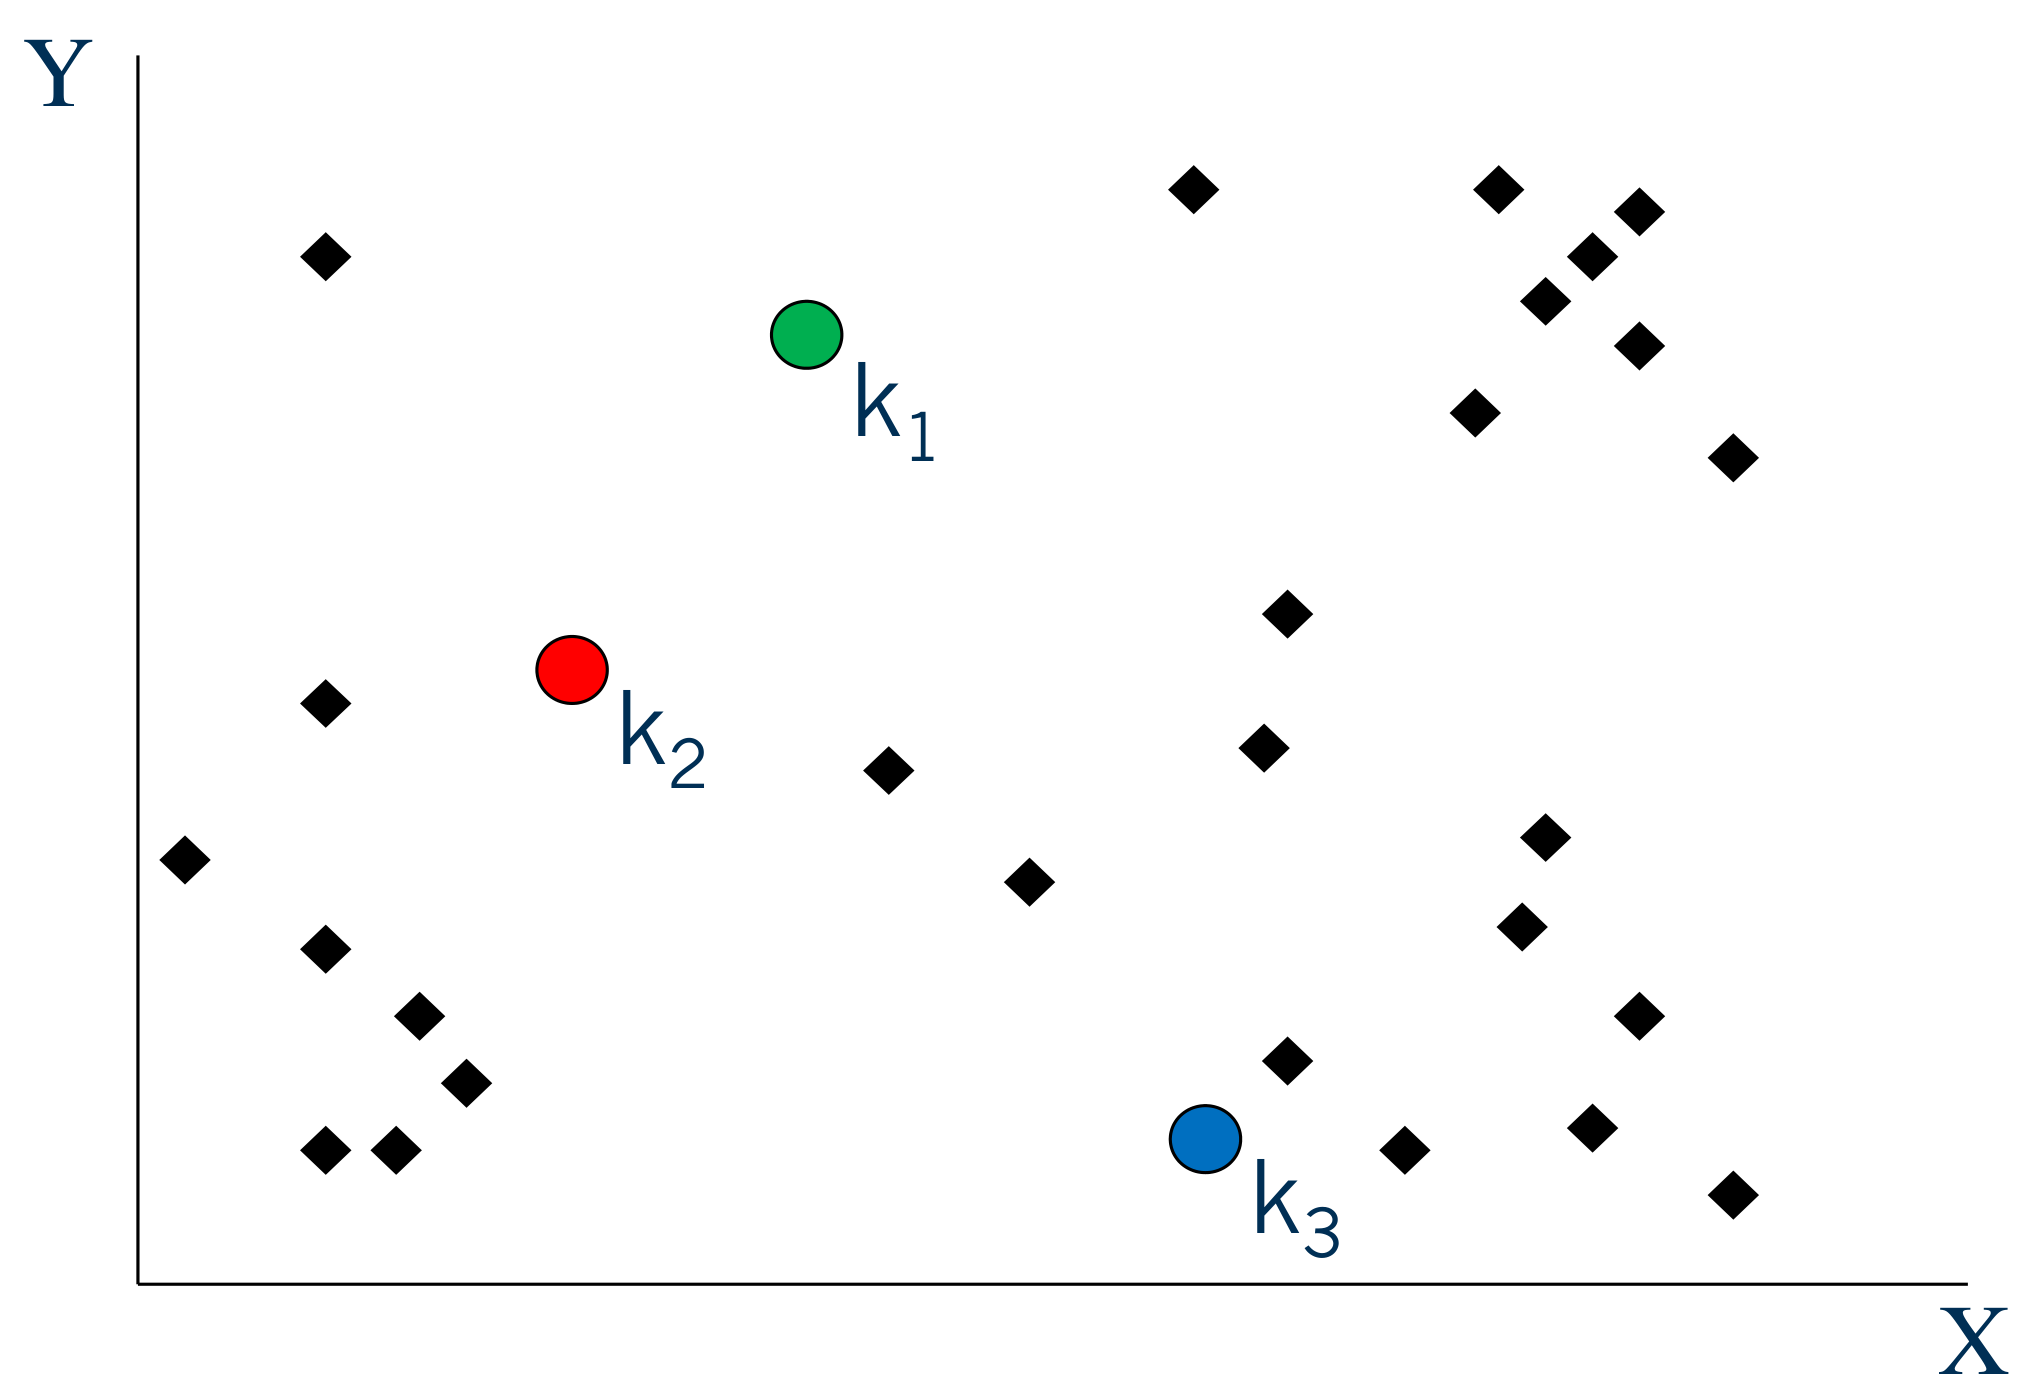
\includegraphics[width=\textwidth,height=4.8cm,keepaspectratio]{images/slide10_kmeans_step.png}
      \end{center}
    \end{column}
  \end{columns}
\end{frame}

% Slide 11: Step 2
\begin{frame}{مثال الگوریتم \lr{$k$-Means}: گام ۲}{\lr{K-Means Example: Step 2}}
  \begin{columns}[T]
    \begin{column}{0.48\textwidth}
      \textbf{تخصیص نقاط به نزدیک‌ترین مرکز:}
      \begin{itemize}
        \setlength{\itemsep}{6pt}
        \item محاسبه فاصله هر نقطه داده تا ۳ مرکز $k_1, k_2, k_3$.
        \item هر نقطه رنگ و برچسب نزدیک‌ترین مرکز به خود را دریافت می‌کند.
        \item خوشه‌های اولیه شکل می‌گیرند.
      \end{itemize}
    \end{column}
    \begin{column}{0.48\textwidth}
      \begin{center}
        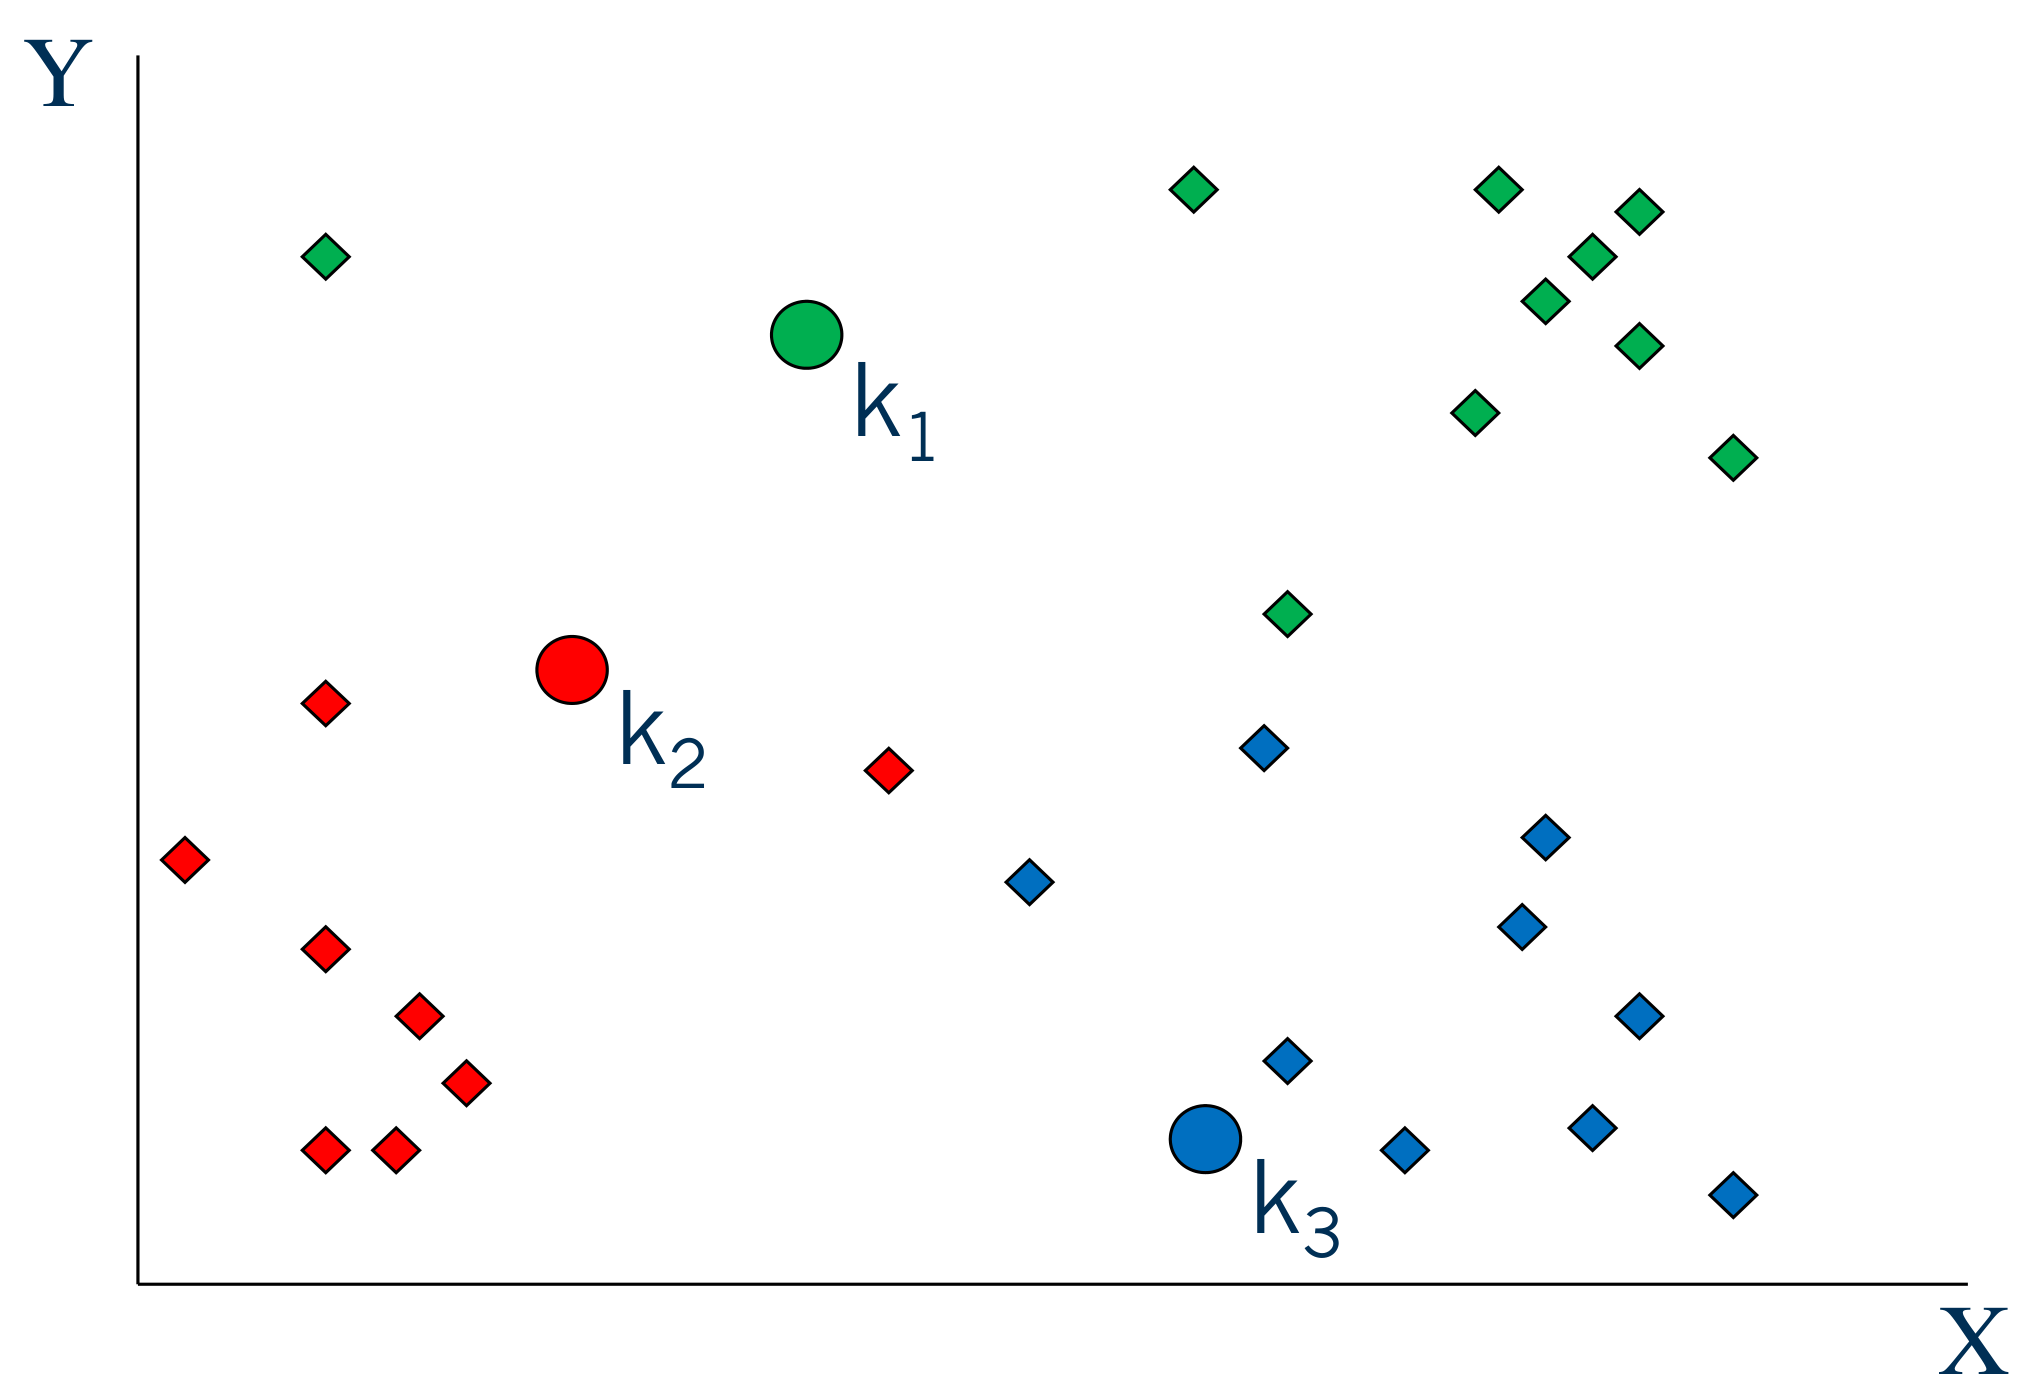
\includegraphics[width=\textwidth,height=4.8cm,keepaspectratio]{images/slide11_kmeans_step.png}
      \end{center}
    \end{column}
  \end{columns}
\end{frame}

% Slide 12: Step 3
\begin{frame}{مثال الگوریتم \lr{$k$-Means}: گام ۳}{\lr{K-Means Example: Step 3}}
  \begin{columns}[T]
    \begin{column}{0.48\textwidth}
      \textbf{به‌روزرسانی موقعیت مراکز خوشه‌ها:}
      \begin{itemize}
        \setlength{\itemsep}{6pt}
        \item محاسبه میانگین مختصات نقاط هر خوشه.
        \item انتقال هر مرکزوار به میانگین جدید نقاط متعلق به آن:
        \begin{itemize}
          \item حرکت $k_1$ به مرکز ثقل نقاط قرمز.
          \item حرکت $k_2$ به مرکز ثقل نقاط آبی.
          \item حرکت $k_3$ به مرکز ثقل نقاط سبز.
        \end{itemize}
      \end{itemize}
    \end{column}
    \begin{column}{0.48\textwidth}
      \begin{center}
        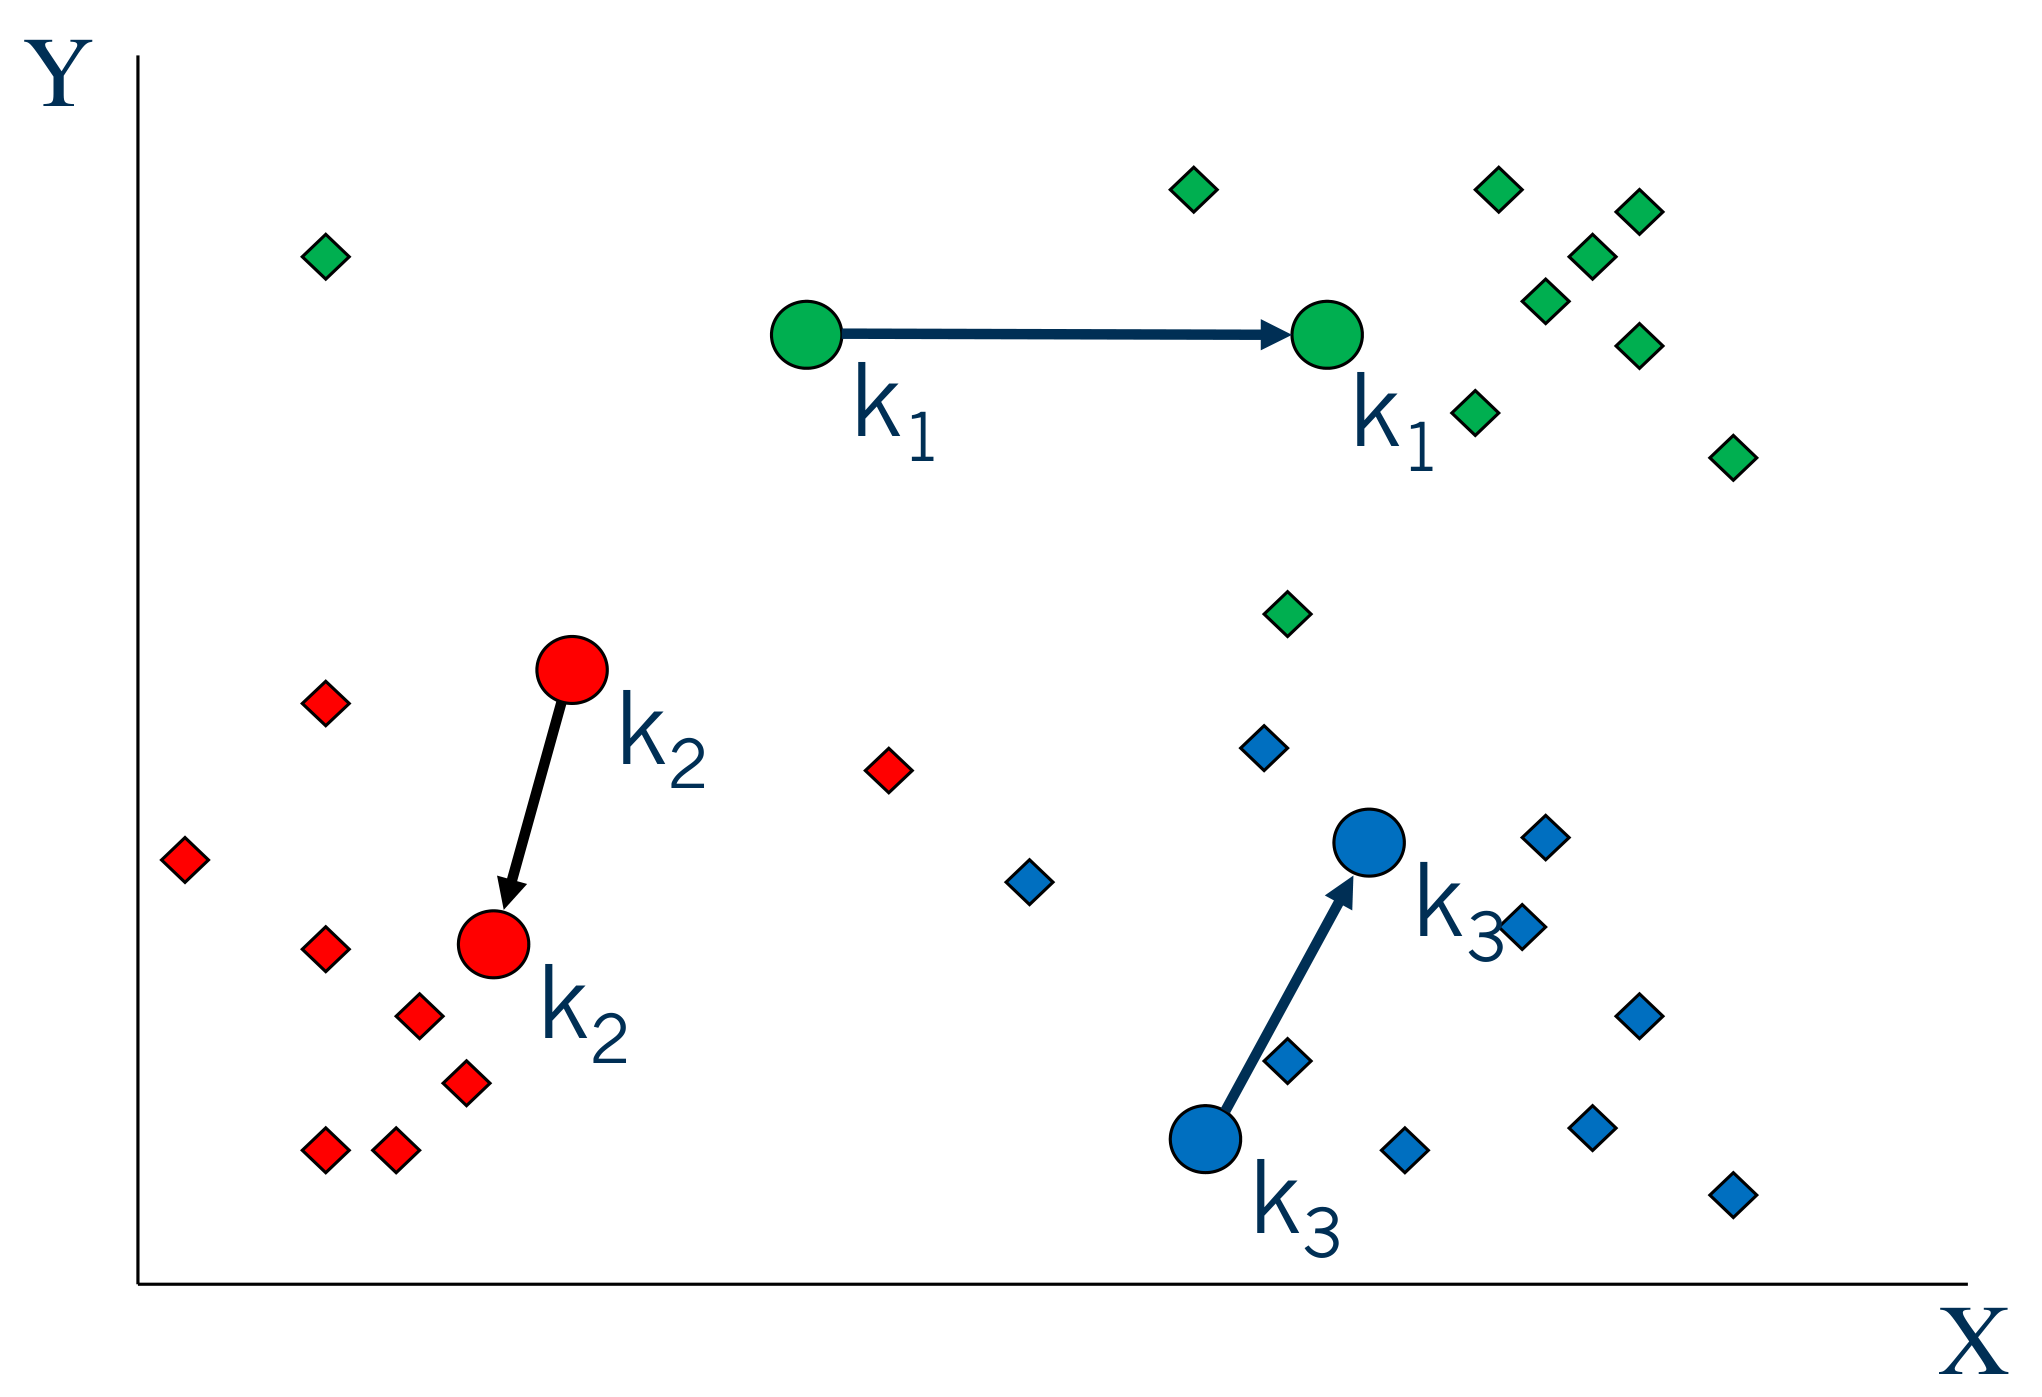
\includegraphics[width=\textwidth,height=4.8cm,keepaspectratio]{images/slide12_kmeans_step.png}
      \end{center}
    \end{column}
  \end{columns}
\end{frame}

% Slide 13: Step 4 - Question
\begin{frame}{مثال الگوریتم \lr{$k$-Means}: گام ۴}{\lr{K-Means Example: Step 4}}
  \begin{columns}[T]
    \begin{column}{0.48\textwidth}
      \textbf{باز‌تخصیص نقاط بر اساس مراکز جدید:}
      \begin{itemize}
        \setlength{\itemsep}{6pt}
        \item بررسی مجدد فواصل: آیا نقطه‌ای وجود دارد که اکنون به مرکز دیگری نزدیک‌تر شده باشد؟
        \item \textbf{پرسش:} کدام نقاط داده تغییر خوشه خواهند داد؟
      \end{itemize}
    \end{column}
    \begin{column}{0.48\textwidth}
      \begin{center}
        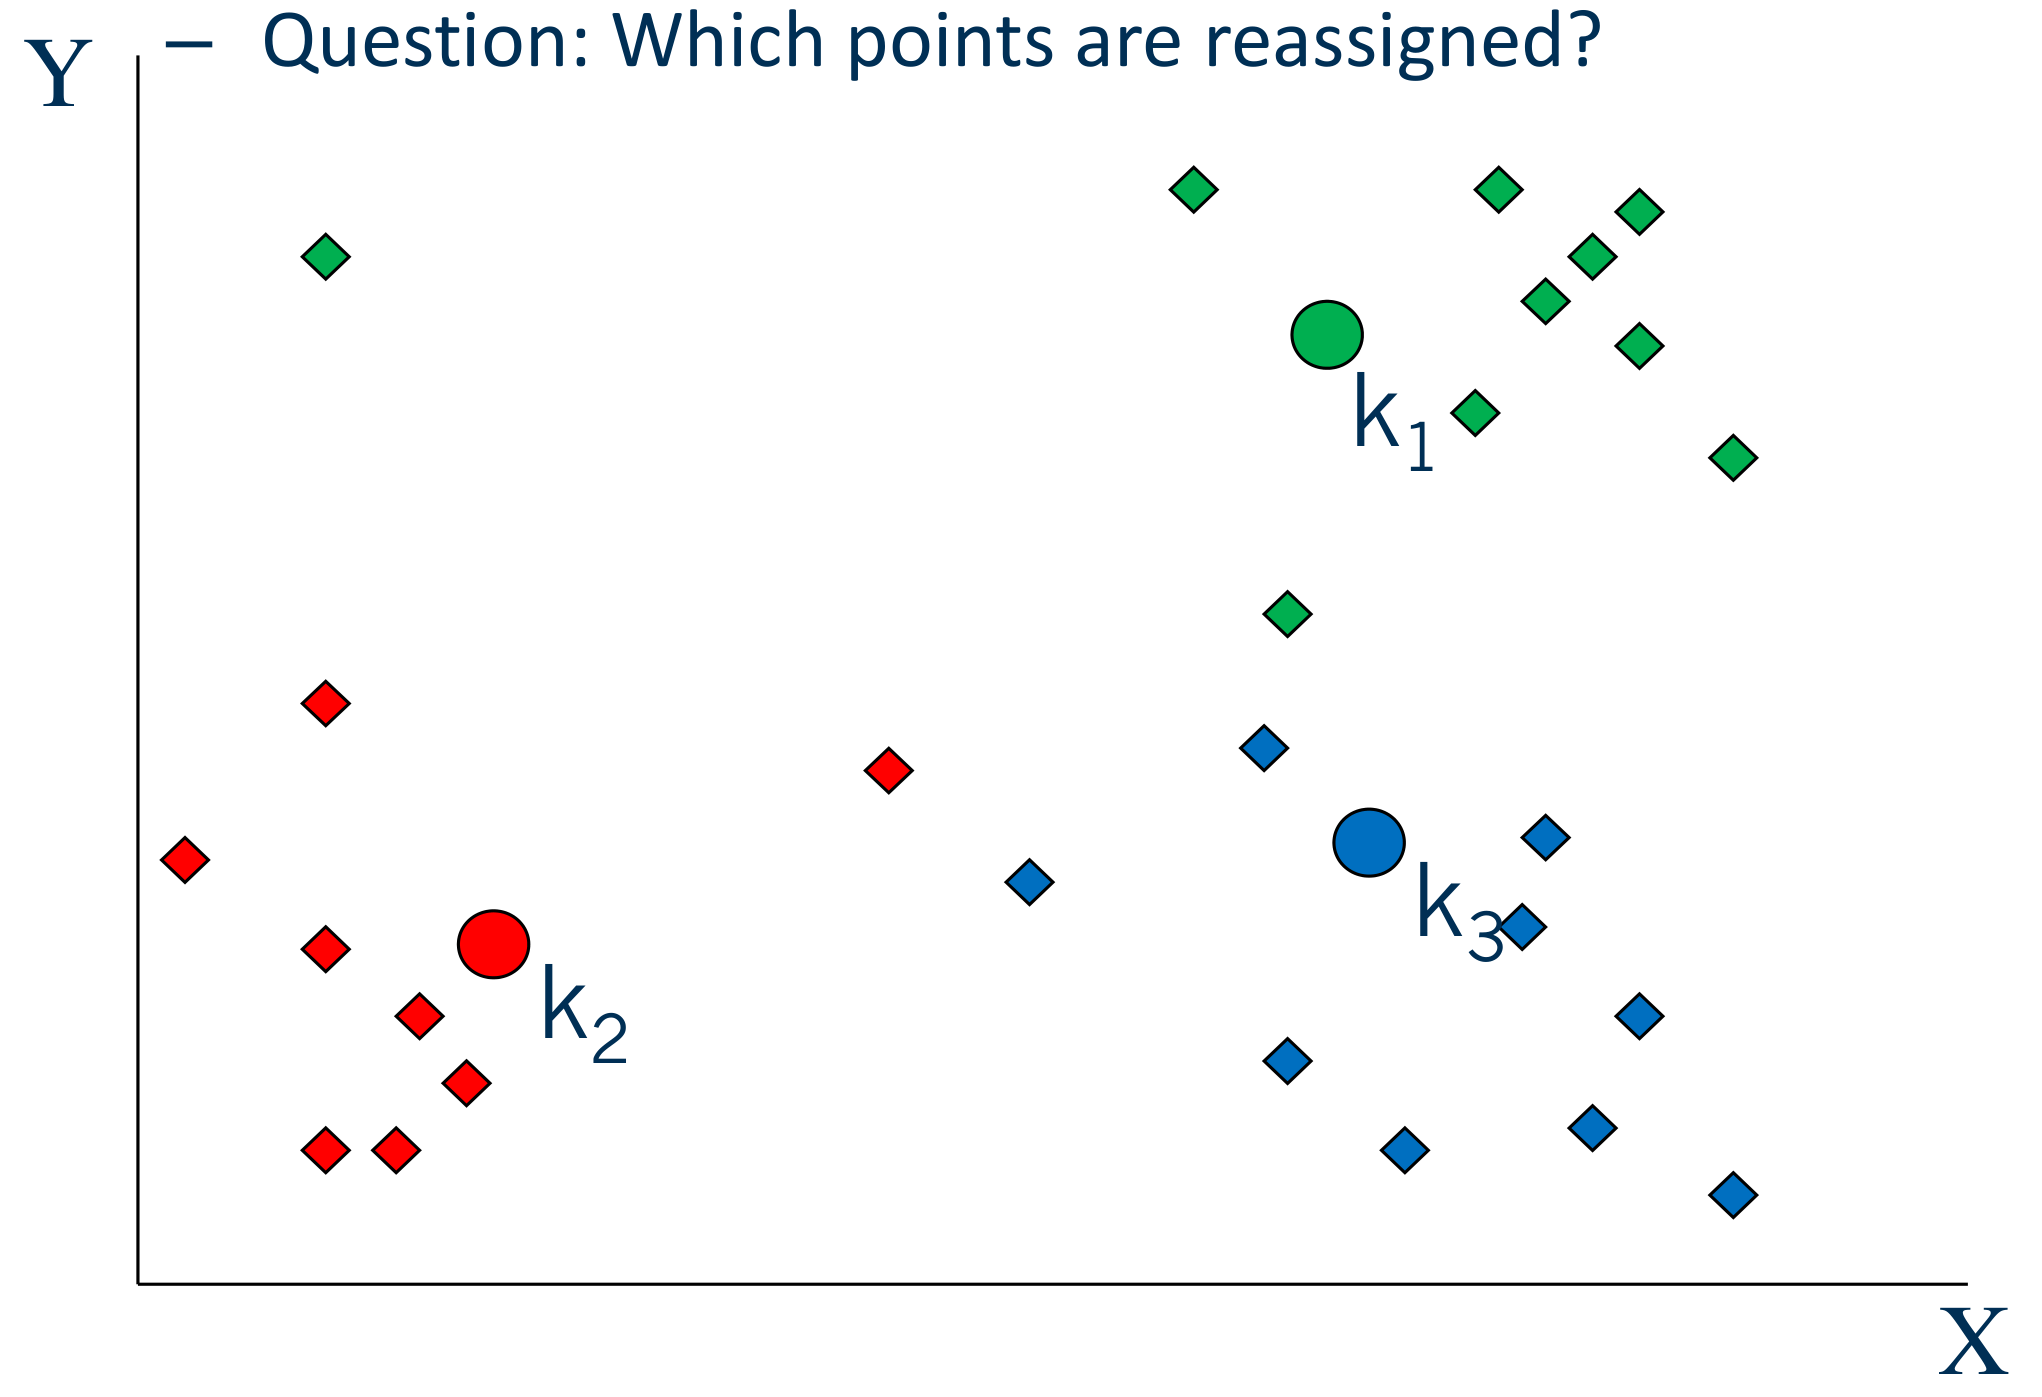
\includegraphics[width=\textwidth,height=4.8cm,keepaspectratio]{images/slide13_kmeans_step.png}
      \end{center}
    \end{column}
  \end{columns}
\end{frame}

% Slide 14: Step 4 - Answer
\begin{frame}{مثال الگوریتم \lr{$k$-Means}: پاسخ گام ۴}{\lr{K-Means Example: Step 4 (Answer)}}
  \begin{columns}[T]
    \begin{column}{0.48\textwidth}
      \textbf{نتیجه باز‌تخصیص نقاط:}
      \begin{itemize}
        \setlength{\itemsep}{6pt}
        \item \textbf{پاسخ:} ۳ نقطه به مرکزوار دیگری نزدیک‌تر شده و برچسب آن‌ها تغییر می‌کند:
        \begin{itemize}
          \item تغییر عضویت از خوشه سبز به آبی یا قرمز بر اساس خطوط مرزی جدید.
        \end{itemize}
        \item تغییر برچسب نقاط نشان‌دهنده نیاز به یک دور دیگر به‌روزرسانی مراکز است.
      \end{itemize}
    \end{column}
    \begin{column}{0.48\textwidth}
      \begin{center}
        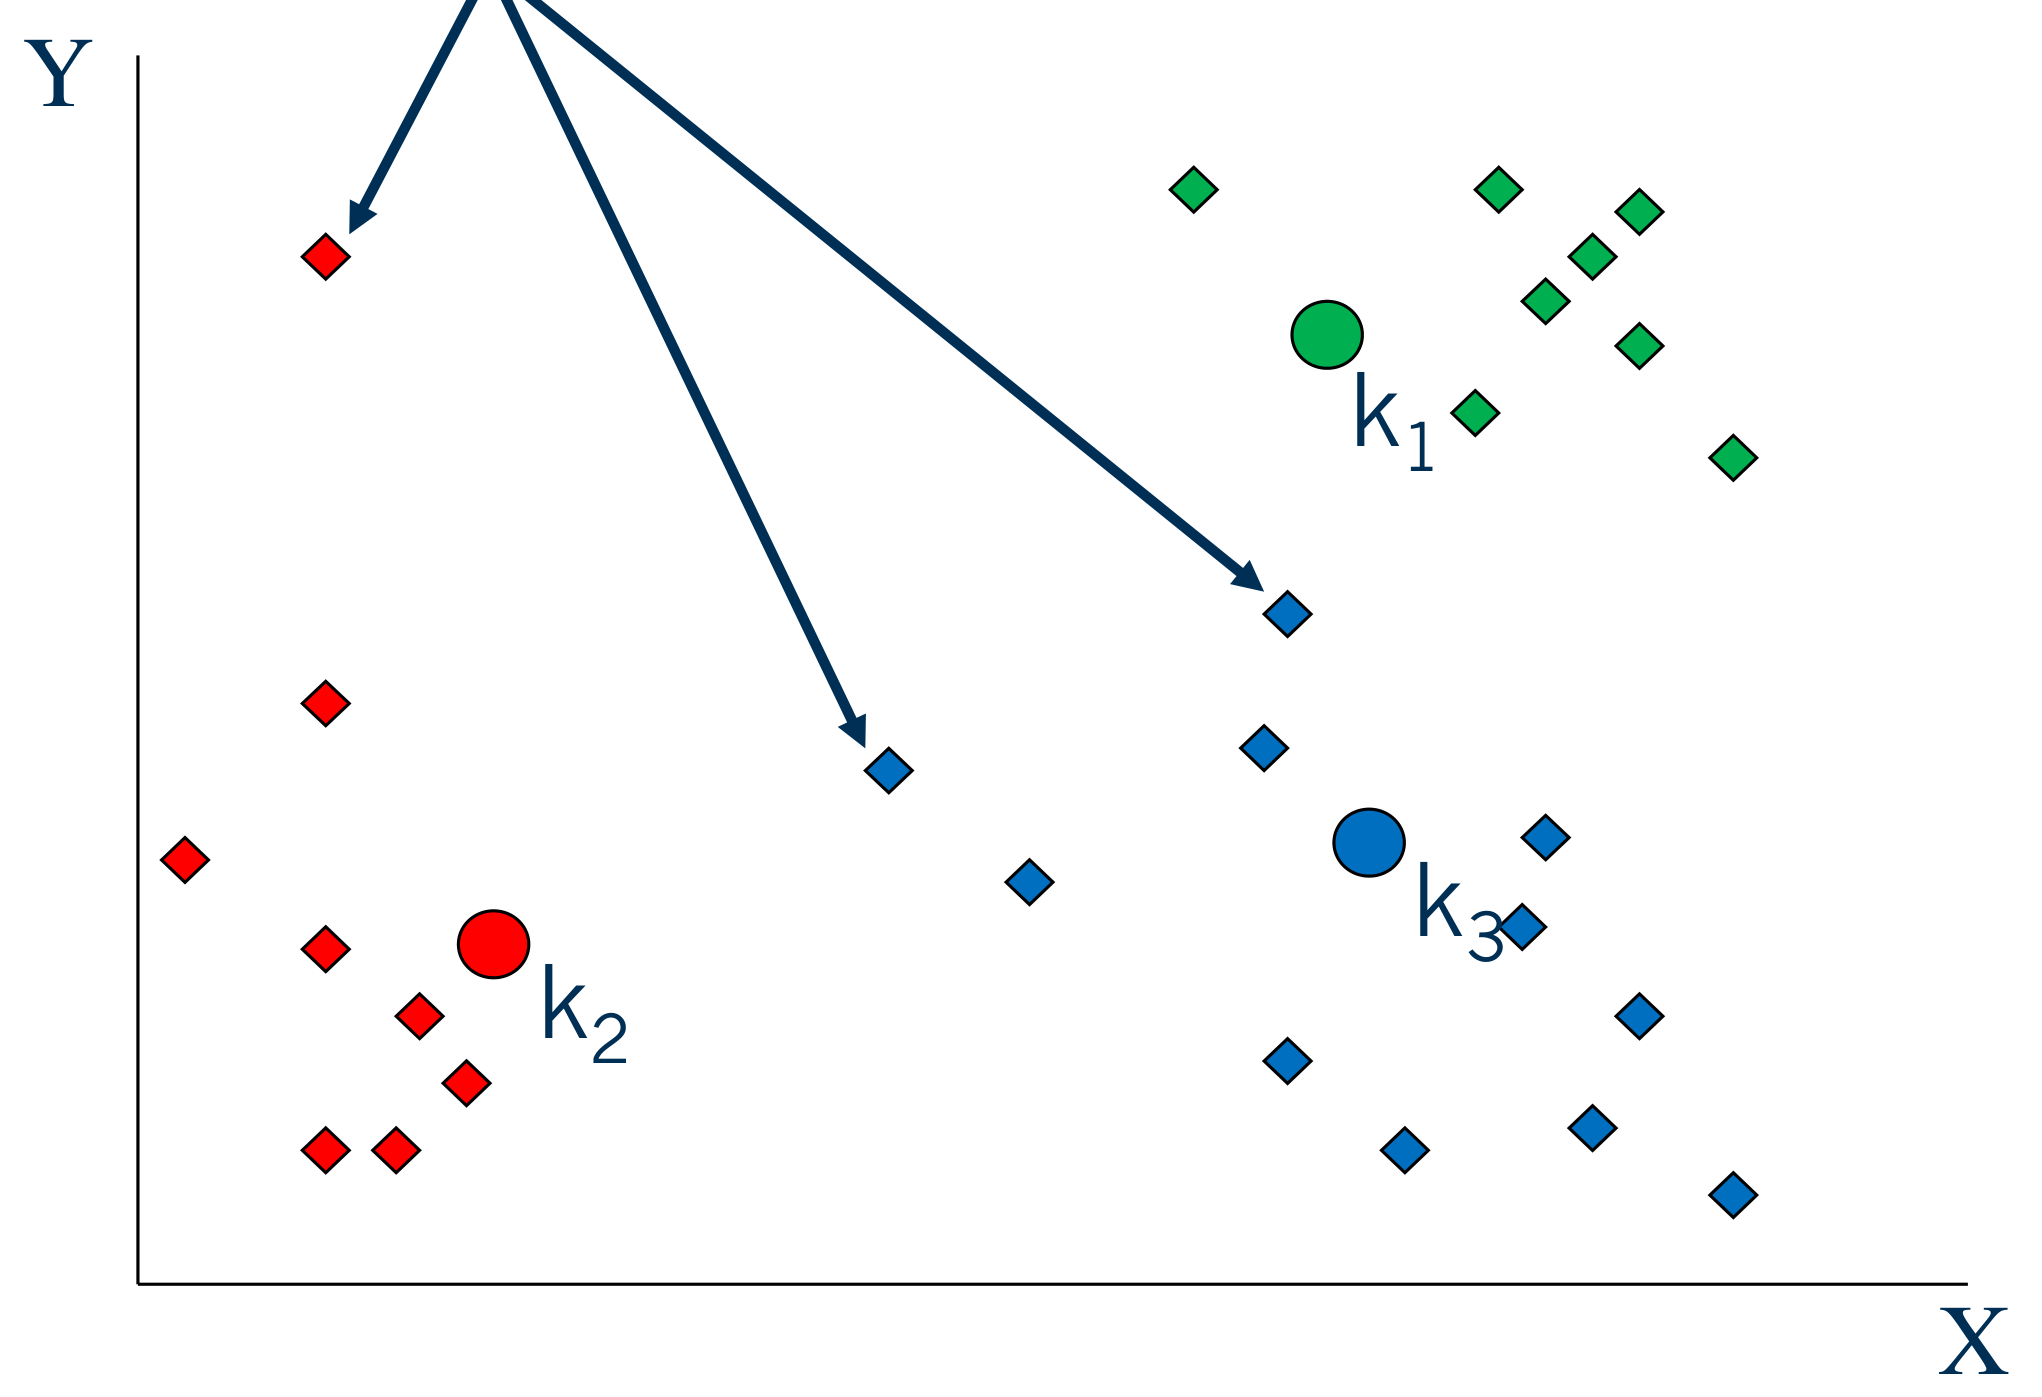
\includegraphics[width=\textwidth,height=4.8cm,keepaspectratio]{images/slide14_kmeans_step.png}
      \end{center}
    \end{column}
  \end{columns}
\end{frame}

% Slide 15: Step 5
\begin{frame}{مثال الگوریتم \lr{$k$-Means}: گام ۵ و همگرایی}{\lr{K-Means Example: Step 5}}
  \begin{columns}[T]
    \begin{column}{0.48\textwidth}
      \textbf{محاسبه مجدد مراکز و همگرایی:}
      \begin{itemize}
        \setlength{\itemsep}{6pt}
        \item مراکز خوشه‌ها مجدداً بر اساس اعضای جدید محاسبه و جابه‌جا می‌شوند.
        \item با انجام گام تخصیص بعدی، هیچ نقطه‌ای تغییر خوشه نمی‌دهد.
        \item الگوریتم به \textbf{حالت پایدار (همگرایی)} می‌رسد و متوقف می‌شود.
      \end{itemize}
    \end{column}
    \begin{column}{0.48\textwidth}
      \begin{center}
        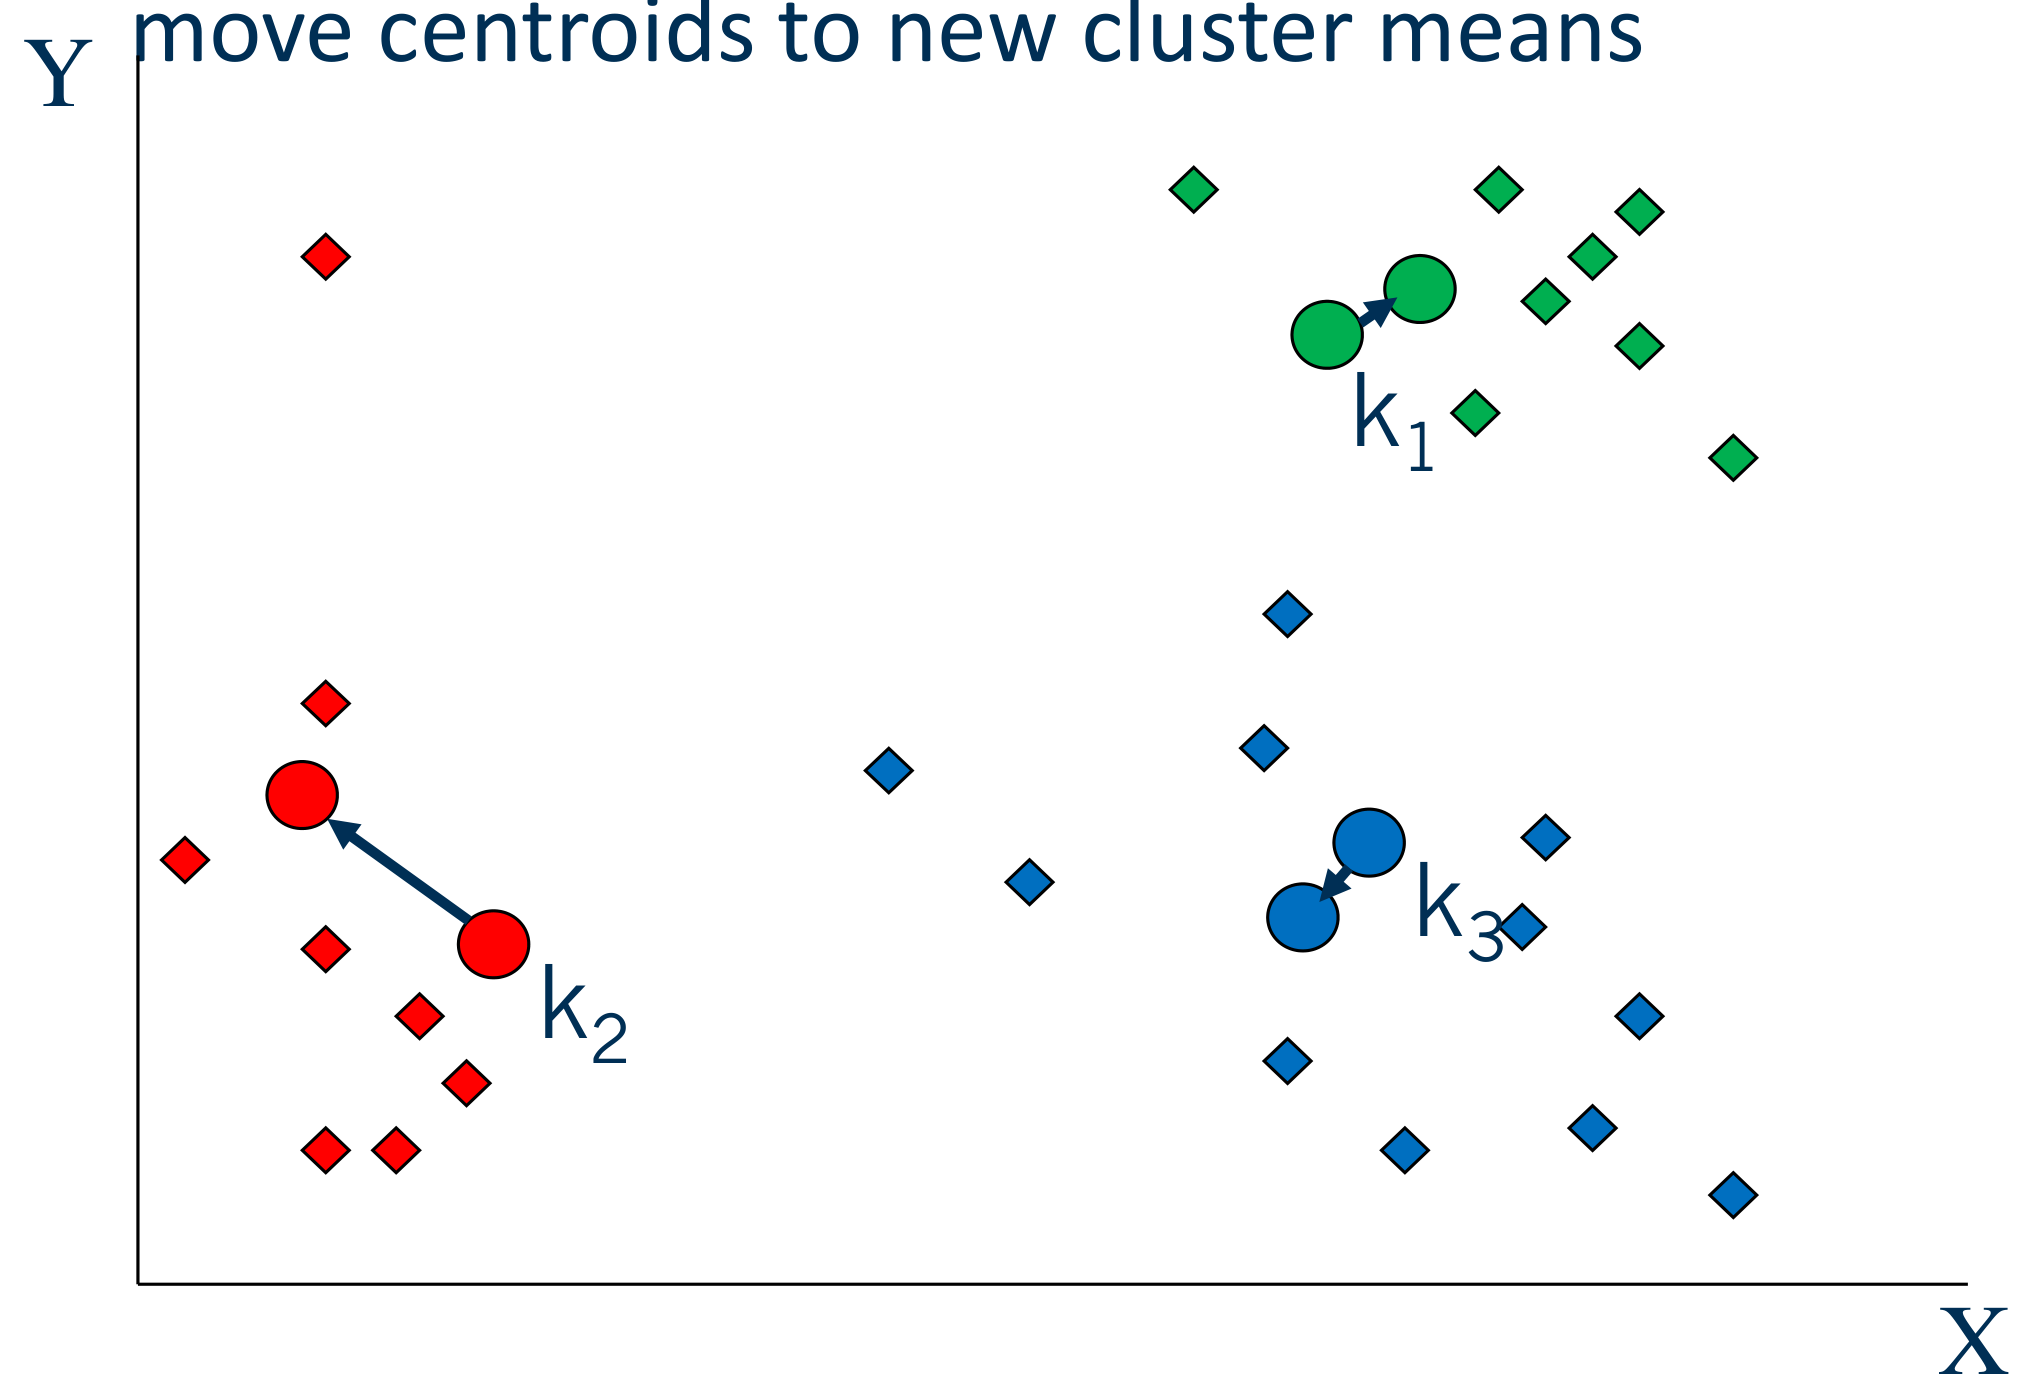
\includegraphics[width=\textwidth,height=4.8cm,keepaspectratio]{images/slide15_kmeans_step.png}
      \end{center}
    \end{column}
  \end{columns}
\end{frame}

% Slide 16: Convergence Criteria
\begin{frame}{معیارهای همگرایی و توقف}{\lr{Convergence Criteria}}
  \begin{itemize}
    \setlength{\itemsep}{6pt}
    \item \textbf{معیار پیش‌فرض همگرایی:}
    \begin{itemize}
      \item عدم تغییر (یا تغییر بسیار ناچیز کمتر از آستانه $\epsilon$) در موقعیت مراکز خوشه‌ها.
    \end{itemize}
    \item \textbf{معیارهای جایگزین توقف:}
    \begin{itemize}
      \setlength{\itemsep}{3pt}
      \item عدم بازتخصیص (یا حداقل جابه‌جایی) نقاط میان خوشه‌ها در دو تکرار متوالی.
      \item رسیدن به سقف مشخصی از تعداد تکرارها \lr{(Max Iterations)}.
      \item کاهش مجموع مربعات خطا \lr{(SSE)} به کمتر از یک حد مشخص (به اسلاید بعدی مراجعه کنید).
    \end{itemize}
  \end{itemize}
\end{frame}

% Slide % Slide 17: Evaluating K-Means: SSE
\begin{frame}{ارزیابی خوشه‌بندی با مجموع مربعات خطا (\lr{SSE})}{\lr{Evaluating K-Means Clusterings: SSE}}
  \begin{itemize}
    \setlength{\itemsep}{4pt}
    \item یکی از پرکاربردترین معیارهای انسجام درون‌خوشه‌ای: \textbf{مجموع مربعات خطا \lr{(Sum of Squared Error - SSE)}}.
    \item برای هر نقطه، خطا برابر با فاصله آن نقطه تا نزدیک‌ترین مرکزوار است. این خطاها به توان دو رسیده و جمع می‌شوند:
  \end{itemize}
  \[
    \text{SSE} = \sum_{j=1}^{K} \sum_{x \in C_j} \text{dist}(x, m_j)^2
  \]
  \begin{itemize}
    \setlength{\itemsep}{3pt}
    \item $C_j$: خوشه $j$-ام.
    \item $m_j$: مرکزوار خوشه $C_j$ (بردار میانگین تمامی نقاط درون $C_j$).
    \item $\text{dist}(x, m_j)$: فاصله اقلیدسی میان نقطه داده $x$ و مرکزوار $m_j$.
    \item \textbf{اصل تصمیم‌گیری:} در میان چند اجرای مختلف با مقدار یکسان $K$، خوشه‌بندی با \textbf{کمترین مقدار \lr{SSE}} برگزیده می‌شود.
  \end{itemize}
\end{frame}

% Slide 18: Illustration: Sum of Squared Error
\begin{frame}{تصویرسازی مفهوم مجموع مربعات خطا}{\lr{Illustration: Sum of Squared Error}}
  \begin{columns}[T]
    \begin{column}{0.55\textwidth}
      \begin{itemize}
        \setlength{\itemsep}{5pt}
        \item \textbf{خوشه‌بندی مطلوب}: \lr{(Good)}
        \begin{itemize}
          \item فواصل نقاط تا مرکزوارها اندک است.
          \item انسجام بالا و \lr{SSE} کمینه.
        \end{itemize}
        \item \textbf{خوشه‌بندی نامطلوب}: \lr{(Not so good)}
        \begin{itemize}
          \item فواصل بیشتر نقاط تا مرکزوارها.
          \item گیر افتادن در بهینه محلی و \lr{SSE} بالاتر.
        \end{itemize}
      \end{itemize}
    \end{column}
    \begin{column}{0.42\textwidth}
      \begin{center}
        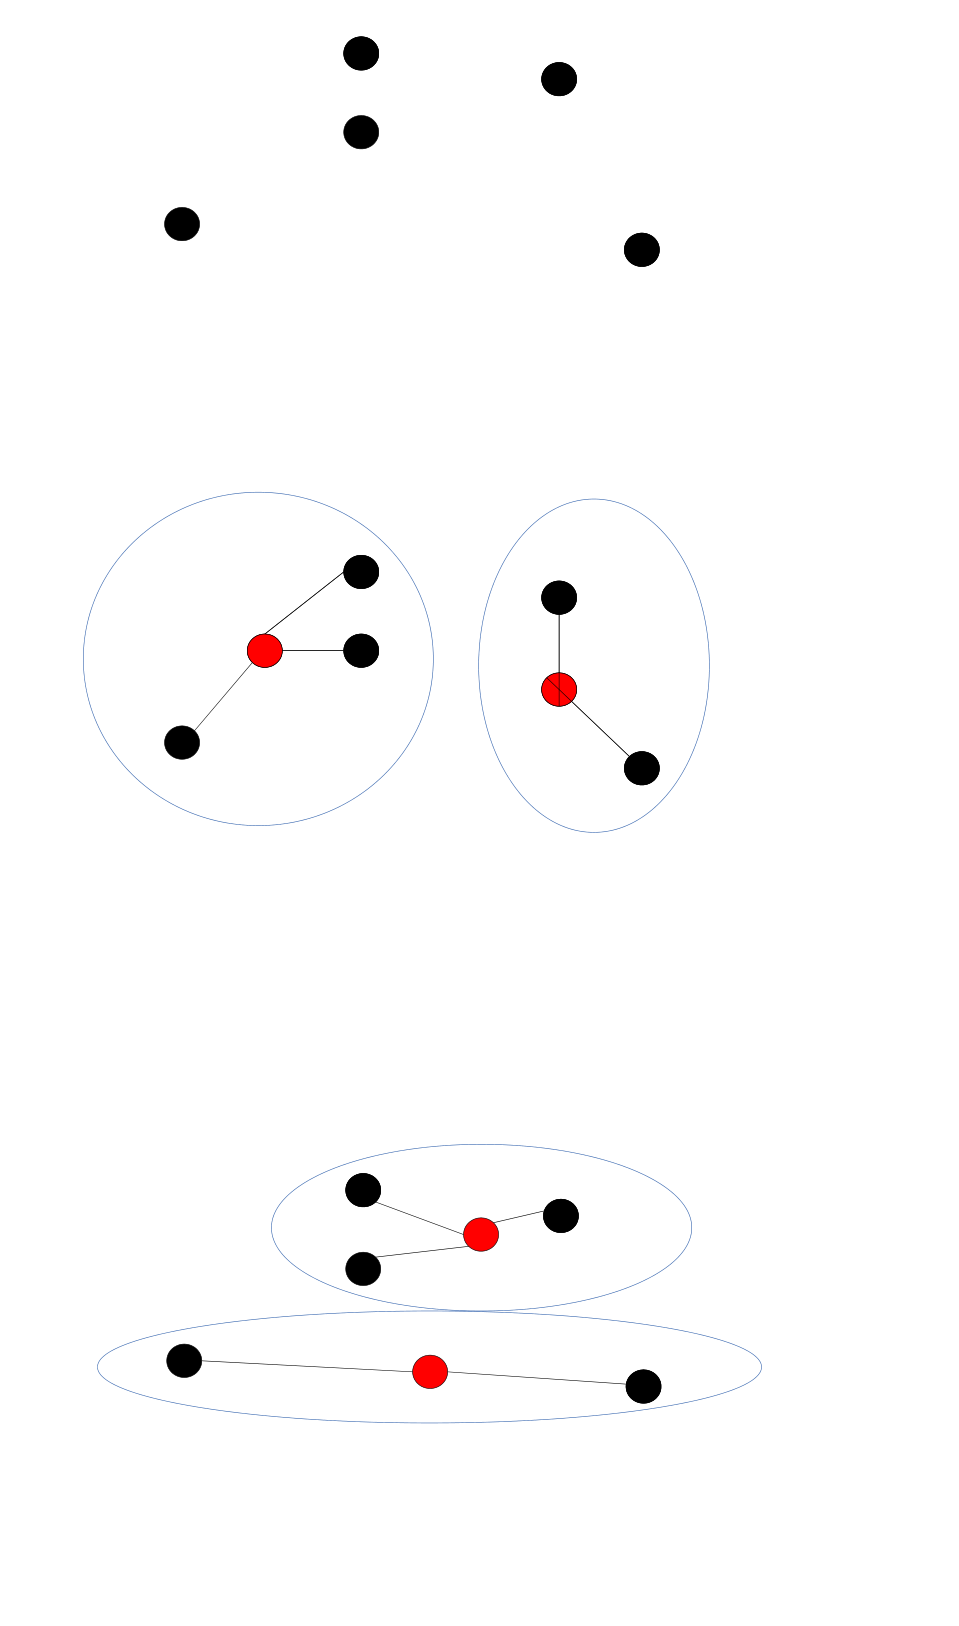
\includegraphics[width=\textwidth,height=4.8cm,keepaspectratio]{images/slide18_sse_diagram_notext.png}
      \end{center}
    \end{column}
  \end{columns}
\end{frame}

% Slide 19: Weaknesses: Initial Seeds
\begin{frame}{نقاط ضعف \lr{$k$-Means}: حساسیت به مراکز اولیه}{\lr{Weaknesses of K-Means: Initial Seeds}}
  \begin{columns}[T]
    \begin{column}{0.5\textwidth}
      \begin{itemize}
        \setlength{\itemsep}{6pt}
        \item نتایج نهایی خوشه‌بندی به‌شدت به \textbf{موقعیت اولیه مراکز تصادفی} بستگی دارد.
        \item انتخاب نامناسب بذرها می‌تواند منجر به خوشه‌بندی‌های بسیار نامطلوب شود.
        \item در تصویر مقابل، دو مرکز در یک خوشه طبیعی و یک مرکز در خوشه‌ای دیگر قرار گرفته‌اند که نتیجه بهینه محلی نامناسب است.
      \end{itemize}
    \end{column}
    \begin{column}{0.48\textwidth}
      \begin{center}
        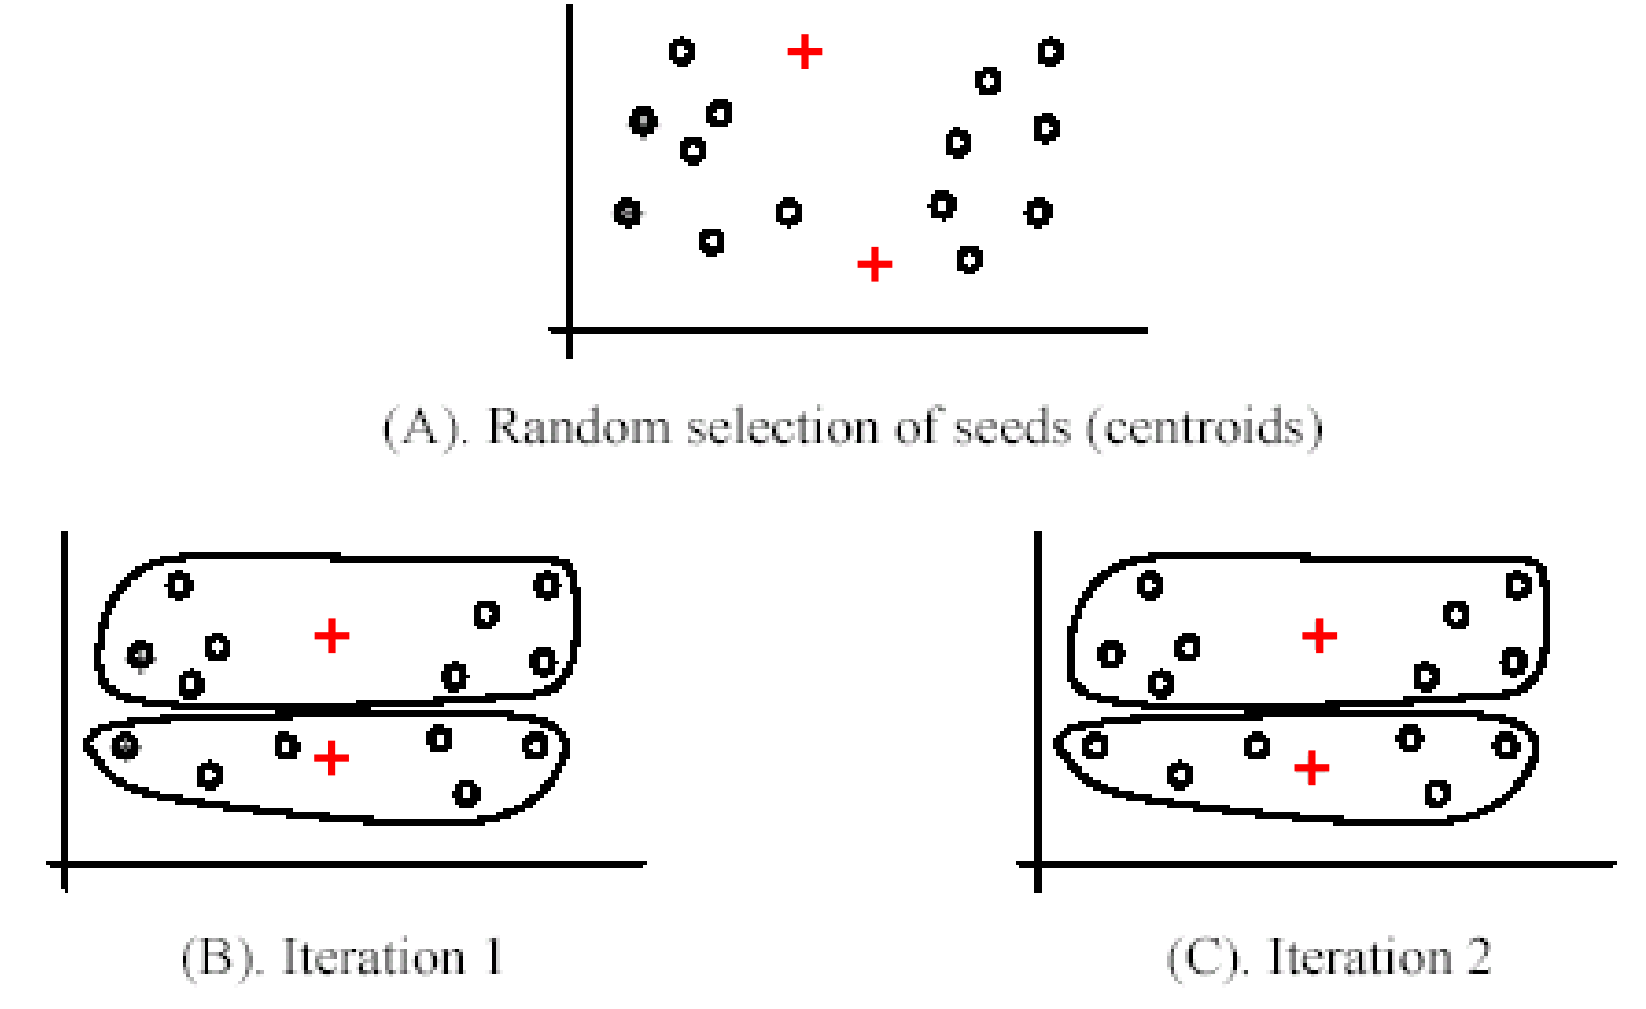
\includegraphics[width=\textwidth,height=4.8cm,keepaspectratio]{images/slide19_initial_seeds.png}
      \end{center}
    \end{column}
  \end{columns}
\end{frame}

% Slide 20: Initial Seeds - Better Result
\begin{frame}{نقاط ضعف \lr{$k$-Means}: بذرهای اولیه مناسب}{\lr{Weaknesses of K-Means: Initial Seeds}}
  \begin{columns}[T]
    \begin{column}{0.5\textwidth}
      \begin{itemize}
        \setlength{\itemsep}{6pt}
        \item اگر مراکز اولیه در نقاط متفاوتی قرار گیرند، الگوریتم به خوشه‌بندی ایده‌آل دست می‌یابد.
        \item در این حالت هر مرکز ثقل به‌درستی درون یکی از ۳ خوشه طبیعی قرار می‌گیرد.
        \item این موضوع نیاز به اجرای مکرر الگوریتم با مقادیر اولیه متفاوت را نشان می‌دهد.
      \end{itemize}
    \end{column}
    \begin{column}{0.48\textwidth}
      \begin{center}
        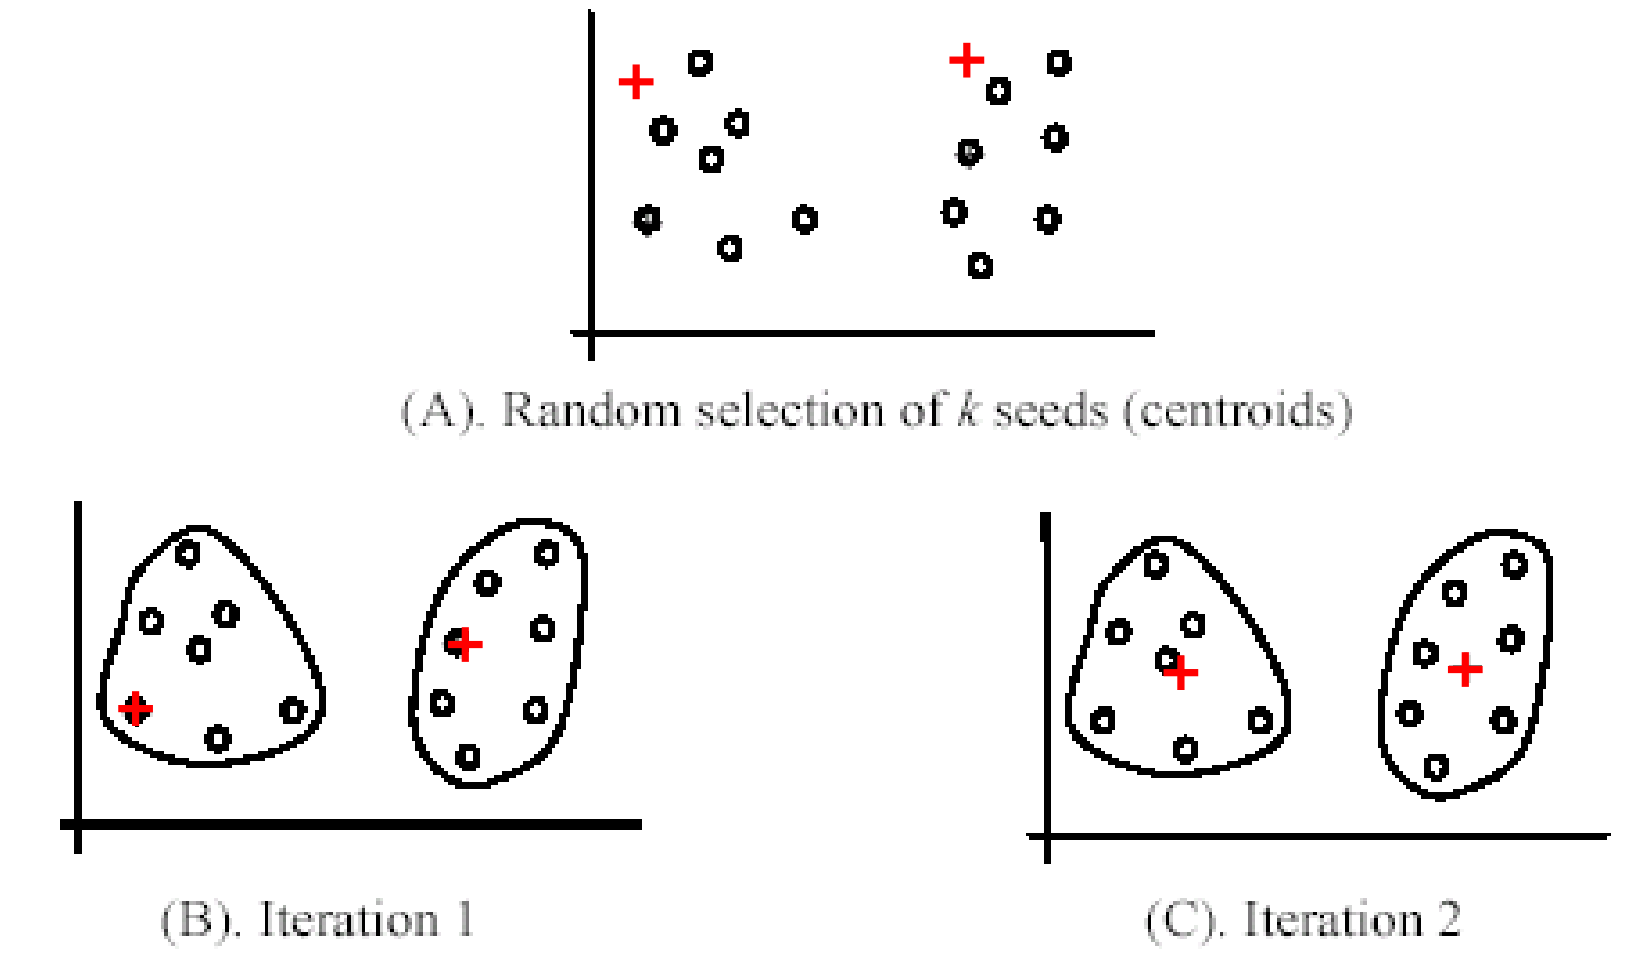
\includegraphics[width=\textwidth,height=4.8cm,keepaspectratio]{images/slide20_initial_seeds_suboptimal.png}
      \end{center}
    \end{column}
  \end{columns}
\end{frame}

% Slide 21: Improving Clustering Results
\begin{frame}{بهبود نتایج و تعیین تعداد خوشه‌ها}{\lr{Improving Clustering Results}}
  \begin{columns}[T]
    \begin{column}{0.58\textwidth}
      \begin{itemize}
        \setlength{\itemsep}{3pt}
        \item \textbf{اجرای چندباره:} \lr{(Restarts)} اجرای مکرر با بذرهای تصادفی مختلف و انتخاب نتیجه دارای کمترین \lr{SSE}.
        \item \textbf{اجرا با مقادیر مختلف $K$:}
        \begin{itemize}
          \item توجه: مقدار \lr{SSE} با افزایش $K$ همواره کاهش می‌یابد (در حالت $K=N$ مقدار $\text{SSE}=0$ است!). بنابراین نمی‌توان مستقیماً \lr{SSE} دو $K$ متفاوت را مقایسه کرد.
        \end{itemize}
        \item \textbf{روش نقطه زانو / آرنج:} \lr{(Elbow / Knee)} انتخاب $K$ در نقطه‌ای که شیب کاهش \lr{SSE} به یکباره کند می‌شود.
        \item \textbf{الگوریتم \lr{X-Means}:} نسخه خودکاری که با $K$ کوچک آغاز کرده و خوشه‌ها را تا رسیدن به تعادل تفکیک می‌کند.
      \end{itemize}
    \end{column}
    \begin{column}{0.4\textwidth}
      \begin{center}
        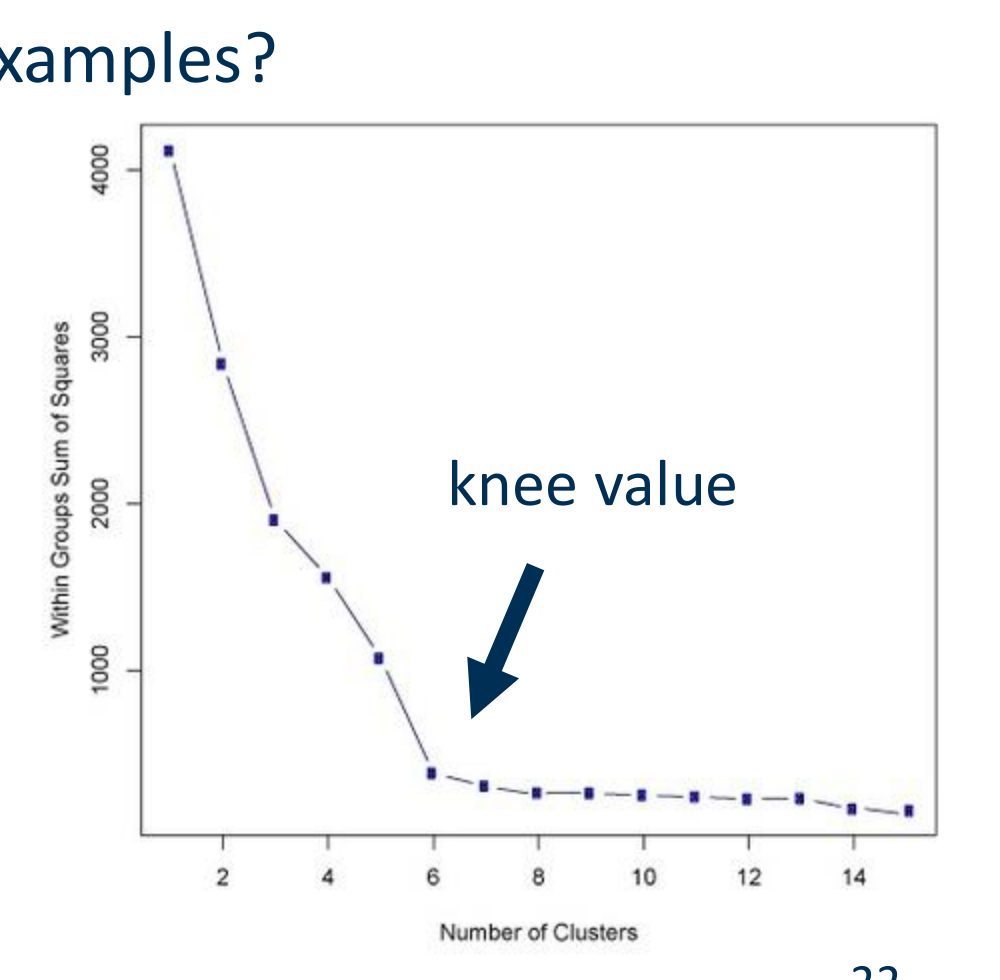
\includegraphics[width=\textwidth,height=4.2cm,keepaspectratio]{images/slide21_elbow_knee.png}
      \end{center}
    \end{column}
  \end{columns}
\end{frame}

% Slide 22: Choosing k - Cluster Evaluation
\begin{frame}{معیارهای ارزیابی خوشه‌بندی در تعیین \lr{$k$}}{\lr{Choosing k -- Cluster Evaluation}}
  \textbf{یادآوری: در خوشه‌بندی به دنبال بهینه‌سازی دو مؤلفه‌ایم:}
  \begin{itemize}
    \setlength{\itemsep}{3pt}
    \item \textbf{انسجام درون‌خوشه‌ای:} \lr{(Cohesion)} نزدیکی و تشابه اشیاء درون یک خوشه (باید بیشینه شود یا فواصل کمینه گردد).
    \item \textbf{تفکیک‌پذیری بین‌خوشه‌ای:} \lr{(Separation)} تمایز و دوری خوشه‌ها از یکدیگر (باید بیشینه شود).
  \end{itemize}
  \vspace{0.2cm}
  \begin{center}
    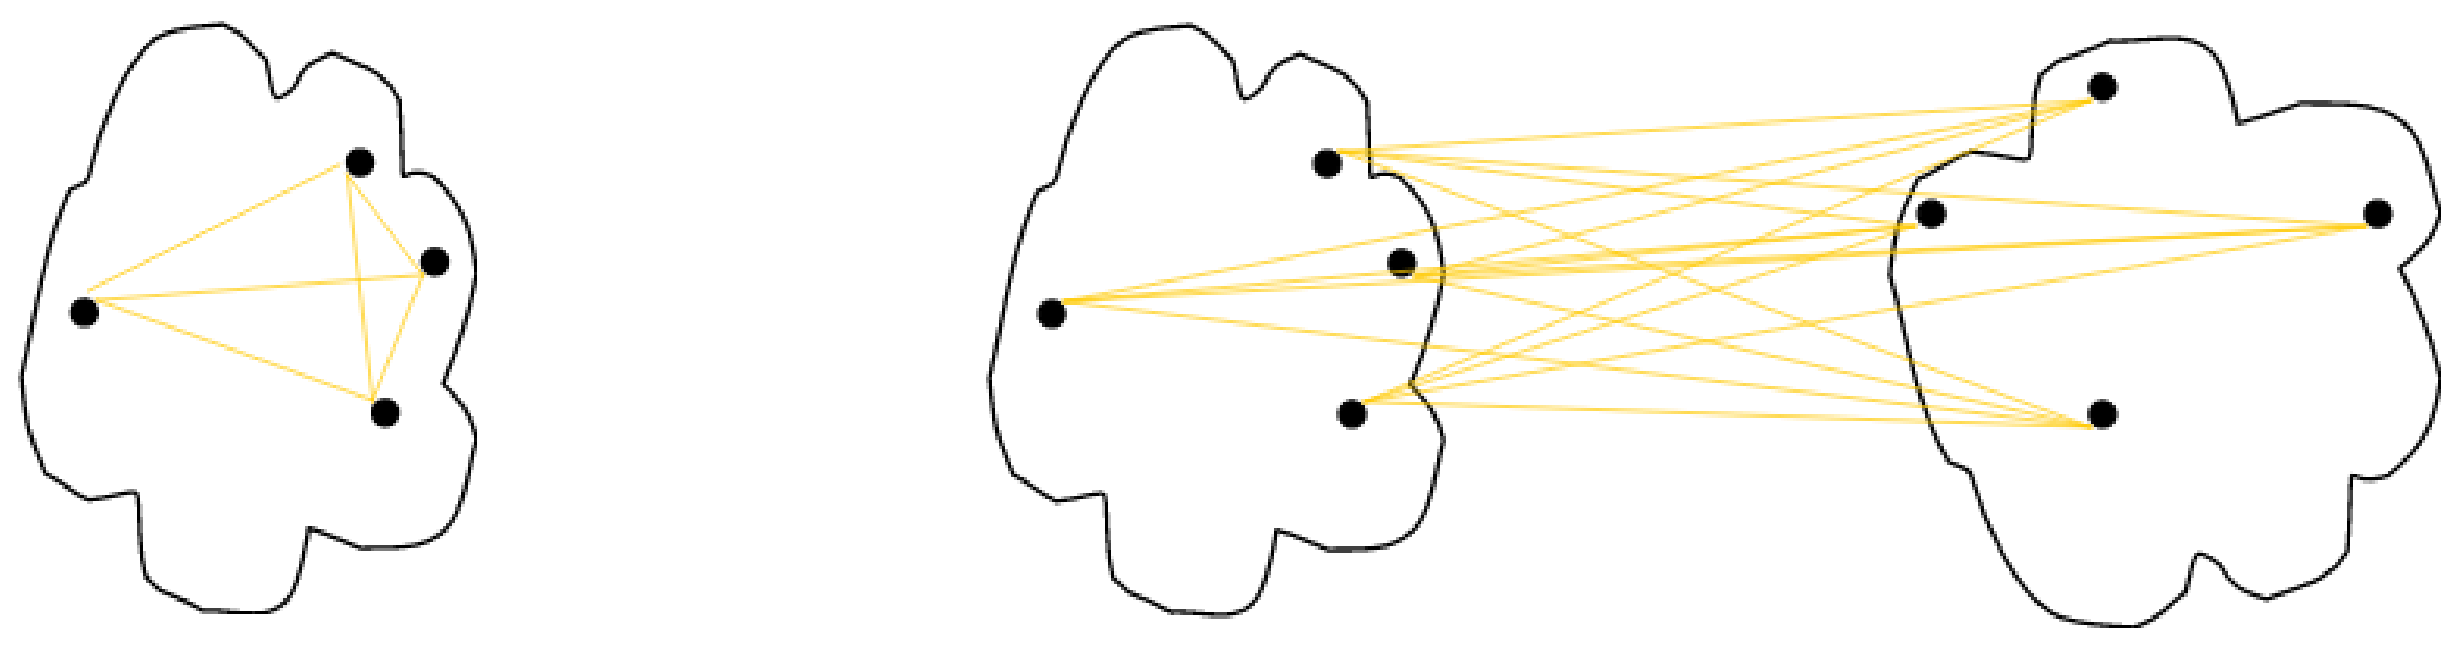
\includegraphics[width=0.92\textwidth,height=2.8cm,keepaspectratio]{images/slide22_choosing_k_metrics.png}
  \end{center}
\end{frame}

% Slide 23: Silhouette Coefficient
\begin{frame}{محاسبه ضریب سیلوئت}{\lr{Silhouette Coefficient}}
  \begin{itemize}
    \setlength{\itemsep}{3pt}
    \item \textbf{انسجام $a(x)$:} میانگین فاصله نقطه $x$ تا تمام نقاط دیگر در همان خوشه.
    \item \textbf{تفکیک $b(x)$:} میانگین فاصله $x$ تا نقاط سایر خوشه‌ها؛ کمترین میانگین در میان خوشه‌ها انتخاب می‌شود:
  \end{itemize}
  \[
    s(x) = \frac{b(x) - a(x)}{\max\{a(x), b(x)\}}
  \]
  \begin{itemize}
    \setlength{\itemsep}{3pt}
    \item دامنه تغییرات: $s(x) \in [-1, 1]$
    \begin{itemize}
      \item $s(x) \approx +1$: بسیار مناسب و تفکیک عالی.
      \item $s(x) \approx 0$: نقطه در مرز میان دو خوشه قرار دارد.
      \item $s(x) \approx -1$: بسیار ضعیف و احتمالاً انتساب نادرست به خوشه.
    \end{itemize}
    \item \textbf{ضریب سیلوئت کل داده‌ها (\lr{SC}):} میانگین ضریب سیلوئت تمامی $N$ نقطه داده:
  \end{itemize}
  \[
    \text{SC} = \frac{1}{N} \sum_{i=1}^{N} s(x_i)
  \]
\end{frame}

% Slide 24: Selecting k Using Silhouette
\begin{frame}{تعیین تعداد خوشه‌ها با ضریب سیلوئت}{\lr{Selecting k Using the Silhouette Coefficient}}
  \begin{columns}[T]
    \begin{column}{0.55\textwidth}
      \textbf{رویکرد اجرایی:}
      \begin{itemize}
        \setlength{\itemsep}{5pt}
        \item اجرای الگوریتم \lr{$k$-Means} با مقادیر مختلف $K$ ($K=2, 3, 4, \dots$).
        \item محاسبه و رسم نمودار ضریب سیلوئت برای هر $K$.
        \item انتخاب $K$ با بیشترین مقدار میانگین سیلوئت.
        \item \textbf{مزیت مهم:} برخلاف \lr{SSE}، ضریب سیلوئت با افزایش طبیعی $K$ لزوماً بهتر نمی‌شود و معیار عادلانه‌ای برای مقایسه است.
      \end{itemize}
    \end{column}
    \begin{column}{0.42\textwidth}
      \begin{center}
        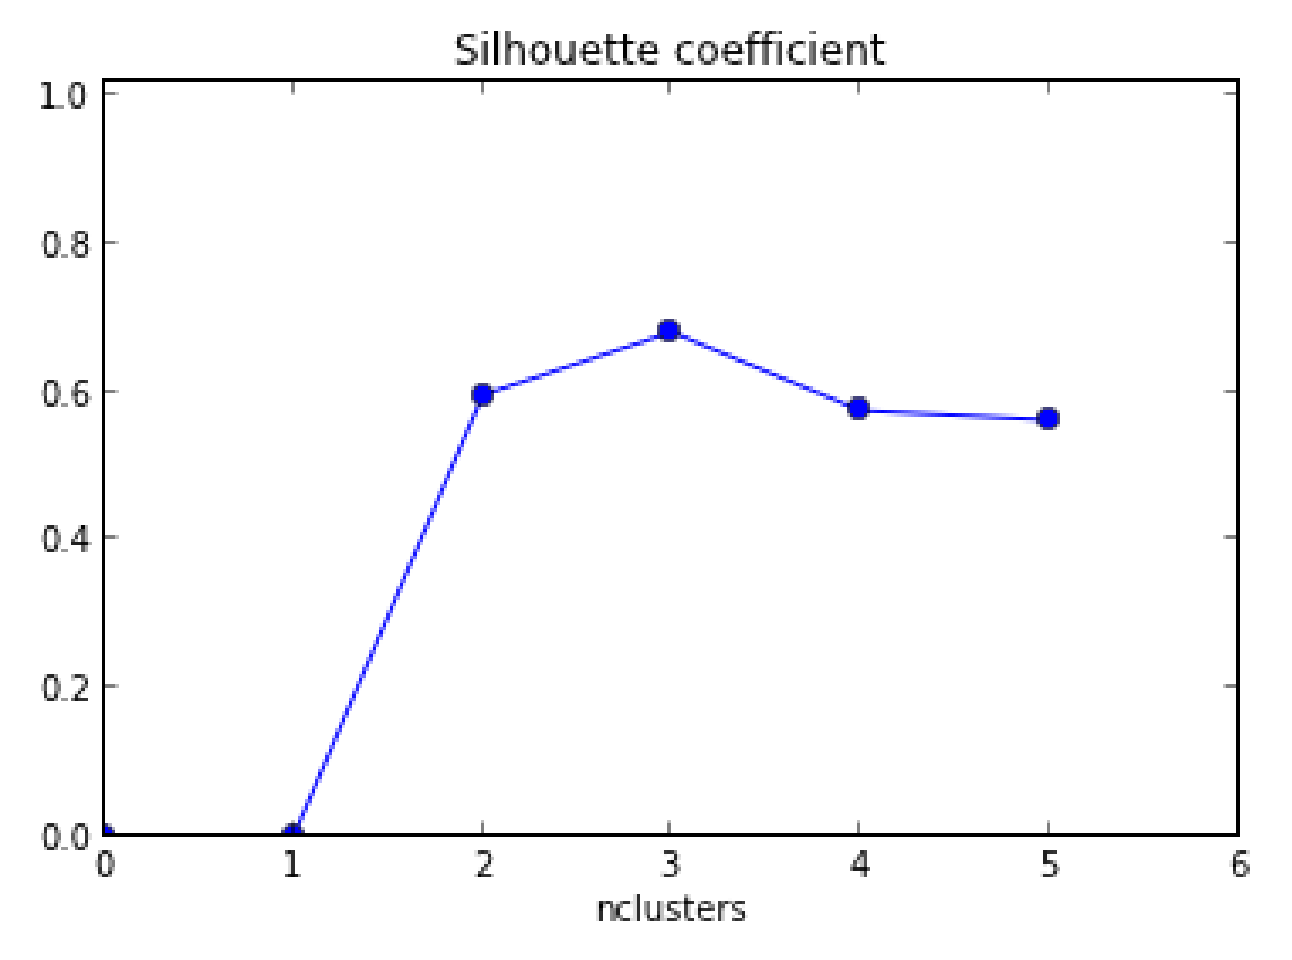
\includegraphics[width=\textwidth,height=4.5cm,keepaspectratio]{images/slide24_selecting_k_scatter.png}
      \end{center}
    \end{column}
  \end{columns}
\end{frame}

% Slide 25: Weaknesses: Outliers
\begin{frame}{نقاط ضعف \lr{$k$-Means}: چالش داده‌های پرت}{\lr{Weaknesses of K-Means: Problems with Outliers}}
  \begin{columns}[T]
    \begin{column}{0.54\textwidth}
      \begin{itemize}
        \setlength{\itemsep}{4pt}
        \item داده‌های دورافتاده مرکزوارها را به سمت خود می‌کشند و خوشه‌بندی را تحریف می‌کنند.
        \item \textbf{راهکارهای مقابله:}
        \begin{itemize}
          \setlength{\itemsep}{2pt}
          \item حذف نقاطی که فاصله زیادی با مراکز دارند (برای اطمینان، می‌توان رفتار آن‌ها را طی چند تکرار رصد کرد).
          \item استفاده از نمونه‌برداری تصادفی \lr{(Random Sampling)} برای تخمین اولیه‌ی مراکز و سپس انتساب مابقی داده‌ها.
        \end{itemize}
      \end{itemize}
    \end{column}
    \begin{column}{0.44\textwidth}
      \begin{center}
        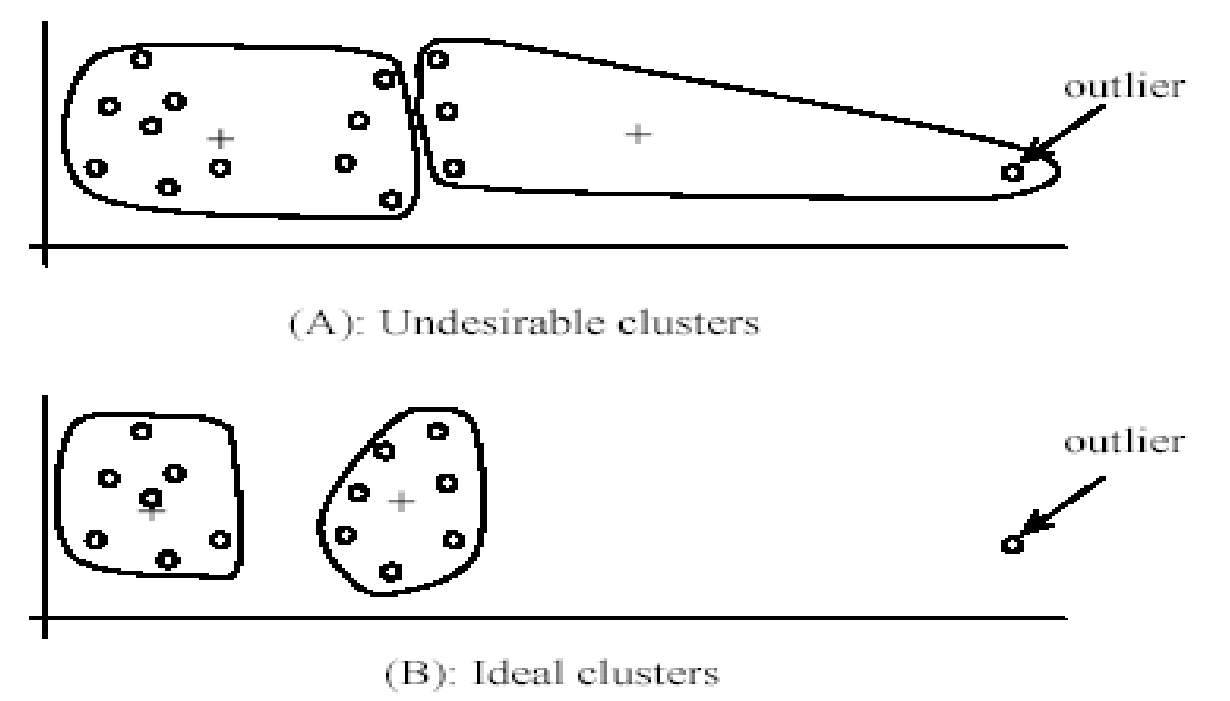
\includegraphics[width=\textwidth,height=4.6cm,keepaspectratio]{images/slide25_kmeans_weaknesses.png}
      \end{center}
    \end{column}
  \end{columns}
\end{frame}

% Slide 26: K-Medoids
\begin{frame}{الگوریتم خوشه‌بندی \lr{$k$-Medoids}}{\lr{K-Medoids Clustering}}
  \begin{itemize}
    \setlength{\itemsep}{5pt}
    \item نسخه‌ای از الگوریتم که به جای \textbf{میانگین}، از \textbf{میانه / مدوئید} \lr{(Medoid)} استفاده می‌کند.
    \item مدوئید مرکزی‌ترین نقطه داده \textbf{واقعی موجود} درون هر خوشه است.
    \item مقاومت و پایداری بسیار بالاتری در برابر داده‌های پرت دارد، زیرا میانه تحت تأثیر مقادیر خیلی بزرگ قرار نمی‌گیرد:
  \end{itemize}
  \vspace{0.2cm}
  \begin{center}
  \begin{tabular}{l c c}
    \toprule
    \textbf{مجموعه داده} & \textbf{میانگین \lr{(Mean)}} & \textbf{میانه \lr{(Median)}} \\
    \midrule
    $\{1, 3, 5, 7, 9\}$ & $5$ & $5$ \\
    $\{1, 3, 5, 7, 1009\}$ & $\mathbf{205}$ & $\mathbf{5}$ \\
    \bottomrule
  \end{tabular}
  \end{center}
\end{frame}

% Slide 27: Summary & Python Implementation
\begin{frame}{جمع‌بندی خوشه‌بندی \lr{$k$-Means} و پیاده‌سازی در پایتون}{\lr{K-Means Summary \& Python Implementation}}
  \begin{columns}[T]
    \begin{column}{0.48\textwidth}
      {\fontsize{8.5}{11}\selectfont
      \textbf{مزایا:}
      \begin{itemize}
        \item ساده و قابل فهم شهودی.
        \item مرتبه زمانی کارآمد: $\mathcal{O}(n \cdot K \cdot I \cdot d)$
        \begin{itemize}
          \item $n$: تعداد داده‌ها، $K$: تعداد خوشه‌ها
          \item $I$: تکرارها، $d$: ابعاد ویژگی‌ها
        \end{itemize}
      \end{itemize}
      \textbf{معایب:}
      \begin{itemize}
        \item نیاز به تعیین قبلی $K$.
        \item اجبار تمام داده‌ها به عضویت در یک خوشه.
        \item حساسیت به نویز و بذرهای اولیه.
      \end{itemize}
      }
    \end{column}
    \begin{column}{0.5\textwidth}
      \begin{latin}
        \begin{minipage}{\textwidth}
          \fcolorbox{codeborder}{codebg}{%
            \begin{minipage}{0.96\textwidth}
              {\fontsize{7.2}{9.5}\selectfont\ttfamily
              \textcolor{mannheimteal}{\# 1. Import KMeans}\\
              \textcolor{blue}{\textbf{from}} sklearn.cluster \textcolor{blue}{\textbf{import}} KMeans\\[0.15cm]
              \textcolor{mannheimteal}{\# 2. Create clusterer}\\
              estimator = KMeans(n\_clusters=3)\\[0.15cm]
              \textcolor{mannheimteal}{\# 3. Fit and predict cluster IDs}\\
              cluster\_ids = estimator.fit\_predict(\\
              \quad dataset[['Att1', 'Att2']]\\
              )
              }
            \end{minipage}%
          }
        \end{minipage}
      \end{latin}
    \end{column}
  \end{columns}
\end{frame}
